\documentclass[12pt,fleqn]{article}\usepackage{../../common}
\begin{document}
Ders 19 

Bu dersten başlayarak ve birkaç ders boyunca çoğu mühendis ve bazı
bilimcinin, onların karşılaştığı türden tüm diferansiyel denklemleri
çözmekte en popüler bulduğu yöntemi göreceğiz. Yöntemin ismi Laplace
Transformu. 

Bu yöntemi kullanmak için birkaç hafta yeterli, ama o zaman bile metot
etrafında belli bir gizem bulutu kalıyor, insanlar tekniğin nereden
geldiğini bir türlü anlayamıyorlar, ve doğal olarak bu onları rahatsız
ediyor.  

Laplace Transformunu anlamanın iyi bir yolu onu üstel seri (power series)
olarak görmektir. Bir üstel seri bildiğimiz gibi şu formdadır

$$ \sum_{0}^{\infty} a_n x^n $$

Bu seriye yapılacak en doğal işlem onu toplamaktır. Sonuç genelde $f(x)$
gibi bir genel tanımla gösterilir, biz burada gelenekten biraz kopacağız,
toplamın $a$ ile ilişkisini iyice belli etmek için $A(x)$ kullanacağız. 

$$ \sum_{0}^{\infty} a_n x^n = A(x)
\mlabel{1}
$$

Bir değişiklik daha: $a_n$ aslında bir ayrıksal dizin içindeki belli $a$
değerleri, bunu da iyice belli etmek için bilgisayar notasyonu kullanalım,
$a_n$, $a(n)$ olsun. 

$$ \sum_{0}^{\infty} a(n) x^n = A(x)$$

Bu şekilde bakınca, üstel serinin yaptığı bir ayrıksal fonksiyonu $a$'yi
(çünkü içinde reel sayılar var, ve bir fonksiyon) belli bir toplam ile
ilintilendirmek. 

$$ a(n) \leadsto A(x) $$

Peki eğer $a(n) = 1$ ise, yani fonksiyon hep aynı sabit değer 1'i
veriyorsa, o zaman toplam ne olur? 

$$ 1 \leadsto \frac{1}{1-x}, \ \ |x|<1 $$

çünkü $a(n) = 1$ ise üstel seri 

$$ = 1 \cdot x + 1 \cdot x^2 + 1 \cdot x^3 + ... $$

$$ = x + x^2 + x^3 + ... $$

olacaktır, ve bu toplam $1/1-x$'e yaklaşır (dikkat: $|x|<1$ olduğu durumda).

Başka bir fonksiyona daha bakalım, $1 / n!$ 

$$ \frac{1}{n!} \leadsto e^x $$

Bu (ilginç) bakış açısında göre, işleme bir ayrıksal fonksiyon giriyor,
dışarıya bir sürekli fonksiyon çıkıyor. Bu arada dikkat, giren $n$ bazlı, çıkan $x$
bazlı. 

Şimdi diyelim ki ayrıksal olan toplam işlemini sürekli hale getirmek
istiyorum. Önce

$$ n = 0,1,2,.. $$

yerine sürekli bir değişken kullanmaya başlarım, mesela

$$ t: 0 \le t \le \infty $$

ki bu $t$ üstteki aralıktaki tüm reel değerleri taşıyabilecek. 

Fakat ayrıksaldan sürekliliğe geçince toplam işlemini kullanamam, onun
yerine entegral kullanmam gerekir. 

$$ \int_0^{\infty} a(t)x^t \ud t $$

Peki bu neyin fonksiyonu acaba? $t$'nin değil çünkü onun ``üzerinden'' entegre
ederek yokediyorum (integrate out), entegrasyon sonrası $t$ kalmıyor. Hayır,
üstteki fonksiyon her $x$ için belli bir değer hesaplayacağına göre, o $x$'in
bir fonksiyonu olmalı.

$$ \int_0^{\infty} a(t)x^t \ud t = A(x)$$

Fakat hala işimiz bitmedi. Hiçbir mühendis, matematikçi üstteki gibi bir
formu kullanmaz, çünkü $x$ baz halde ve bu tür ifadeler türev alırken,
entegrasyon yaparken problem çıkartabilir. Daha iyi bir baz $e$ olur, $e$
bazlı türev almayı, entegrasyon yapmayı herkes sever [çünkü çok kolay]. 

$$ x = e^{\ln x} $$

$$ x^t = (e^{\ln x})^t $$

Bir nokta daha: eğer $x > 1$ ise üstteki entegralin bir değer yaklaşması
(converge) çok zordur, çünkü entegral üst sınırında $\infty$ var, bu tür
entegraller dikkatli muamele ister. O zaman şu şartı koyarım, $0 < x < 1$. 

Eğer  $0 < x < 1$ olacak ise, $\ln x < 0$ demektir. 

Tabii kimse $\ln x$'i bir değişken olarak kullanmaz, 

$$ s = \ln x $$

ve negatif değişkenlerle uğraşmak istemediğimiz için 

$$ -s = -\ln x $$ 

yaparız, ki hep pozitif olan $-s$ ile iş yapabilelim. 

Tüm bunlar kozmetik değişiklikler bu arada, sembolik olarak bu işlemi
hoşumuza giden bir şeye döndürmek için yaptıklarımız. 

Entegrali tekrar yazalım şimdi. Öncelikle kimse fonksiyon olarak $a(t)$
ismini kullanmaz, ona $f$ diyelim. 

$$ \int_0^{\infty} f(t)(e^{-s})^t \ud t = ..$$

Üstünü almak, kurallara göre çarpıma dönüştüğüne göre

$$ \int_0^{\infty} f(t)e^{-st} \ud t = ..$$

Fonksiyon neye eşit? $A(x)$, $x$'in fonksiyonu idi, ama şimdi $s$
kullanıyoruz, o zaman 

$$ \int_0^{\infty} f(t)e^{-st} \ud t = F(s)$$

Nihai formül ustteki. Ve tekrar vurgulayayım, bu formül ayrıksal üstel seri
(1)'in analog versiyonundan ibaret. İşte Laplace Transformu budur. Bu
operasyonun en alışılmadık tarafı içeri $t$'nin fonksiyonun girmesi, ama
dışarı $s$'in fonksiyonun çıkması. Kıyasla operatörlerde böyle değildi,
diferansiyel operatöründe mesela $3x$ giriyor, dışarı $3$ çıkıyor, ama
burada işler böyle değil, bu karışıklık yaratıyor. Ama vurgulamak gerekir
ki Laplace Transformu adı üstünde bir transformdur, değişkenin değişmesinin
sebebi burada. 

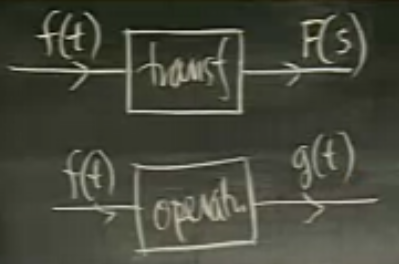
\includegraphics[height=3cm]{19_1.png}

Laplace için kitabımızın kullandığı notasyon 

$$ \mathcal{L}(f(t)) = F(s) $$

Fakat bazen bu notasyonu kullanmak çok zor oluyor, bir sürü parantez üst
üste biniyor, vs. O durumlarda şu yeterli

$$ f(t) \leadsto F(s) $$

Tabii lineerlik kuralını da üstteki ile ifade etmek zor, onun için
$\mathcal{L}$ daha iyi, 

$$ \mathcal{L}(f+g) = \mathcal{L}(f) + \mathcal{L}(g) $$

Sabitle çarpım kural 

$$ \mathcal{L}(cf) = c \mathcal{L}(f)  $$

Lineerlik kuralı işliyor çünkü entegraller bağlamında düşünürsek,
entegrallerin toplamı aynı entegral altında gruplanabilir, yani bu kural
işliyor çünkü entegralin kendisi de lineer bir operatör. 

Eh artık ise koyulalım. Mesela bildik bazı fonksiyonların Laplace
transformunu bulalım. 

Örnek

$$ 1 \leadsto ? $$

$$ \int_0^{\infty} e^{-st} \ud t $$

Dikkat, bu entegral uygun olmayan bir (improper) entegral. Bu tür
entegrallerin tanımına bakalım

$$ \lim_{R \to \infty}  \int_{0}^{R} e^{-st} \ud t  $$

Önce şu entegrali hesaplayalım, 

$$  \int_{0}^{R} e^{-st} \ud t $$

$t$'ye göre entegral alıyoruz, o zaman $s$ bir sabit gibidir. 

$$  = \frac{ e^{-st}}{-s}  \bigg|_{0}^{R} $$

$$ = \frac{e^{-sR} - 1}{-s} $$

O zaman 

$$ \lim_{R \to \infty}  \int_{0}^{R} e^{-st} \ud t  = 
\lim_{R \to \infty} \frac{e^{-sR} - 1}{-s}  = \frac{1}{s}
$$

Yani 

$$ 1 \leadsto \frac{1}{s} $$

Bu doğru mu? Hayır değil. Bir hata yaptık, daha doğrusu bir şeyi
atladık. Limit ifadesindeki $e^{-sR}$ sıfıra gider, sadece ve sadece $s >
0$ ise. Sonucun tam hali 

$$ 1 \leadsto \frac{1}{s}, \ \ s > 0 $$

Ama diğer yandan ``ya $s < 0$ ise o zaman Laplace Transformu nedir?''
sorusunun da anlamı yoktur. 1'in Laplace transformu alttaki fonksiyondur,
bu fonksiyonun eksi bölgesinde karşılığı yoktur. 

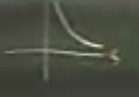
\includegraphics[height=2cm]{19_2.png}

Örnek 

$$ e^{at} \leadsto ? $$

Bu arada insanlar Laplace transform tekniğini şimdiye kadar pek çok kez
gördüğümüz türden fonksiyonlar üzerinde kullanırlar hep, üstel fonksiyonlar,
polinomlar, sinüs, cosinüs ifadeleri, kompleks sayılar gibi. Diğer türden
şeylerde .. onu kullanmazlar. Bu hayal kırıklığı yaratmasın, ODE çözerken
Laplace tekniği bazı işleri diğer kullandığımız tekniklerden çok daha iyi
yapar. Neyse Laplace'in avantajlarına ileride daha belirgin vurgu
yapacağız. Örneğimize dönelim. 

Aslında daha genel bir duruma bakalım, şu ifadenin

$$ e^{at}f(t) $$

Laplace transformunu yapacağız, ve bunu $f(t)$'nin transformu bilindiği
durum için yapacağız, üstteki blok ifade için genel bir formül üreteceğiz,
ve onu başarınca, $e^{at}$ ifadesi $e^{at} \cdot 1$ olarak görülebilir, eh
1'in transformunu zaten biliyoruz, o zaman genel formül üzerinden $e^{at}$'in
transformunu hemen buluruz. Genel formülün transformu

$$ \int_0^{\infty} e^{at} f(t)e^{-st} \ud t $$

İki üstel ifadeyi birleştirelim, ve öyle yapalım ki $f(t)$'in transformu
bir şekilde formülde olsun. Ulaşmak istediğim nokta 

$$ \int_0^{\infty} f(t)e^{-( ... )t } \ud t $$

şeklinde, eğer eksi bu şekilde dışarıda kalacaksa, geri kalanlar neye
benzer? 

$$ \int_0^{\infty} f(t)e^{-(s-a)t } \ud t $$

Bu nedir? Bu da bir Laplace transformudur! Eğer $-a$ orada olmasaydı, geri
kalanlar $f(t)$'nin transformu olacaktı. O zaman 

$$ = F(s-a) $$

Şartları koyalım, üstteki durumda $s-a > 0$ olmalı, o zaman $s > a$
olmalı. 

$F$ içinde $-a$ sonucu bir tür ``kaydırma'' gibi duruyor, zaten bu genel
formülün ismi ``üstel kaydırma kuralı (exponential shift
law)''. Mühendisler bu kuralı çok kullanırlar. 

$e^{at}$'ye dönelim. 1'in transformu $1/s$ ise, kaydırma kuralıyla

$$ e^{at} \leadsto \frac{1}{s-a} $$

Peki transform edilmek istenen sinüs ve cosinüs olduğu durumlarda ne
yaparız? Hatırlayalım, $\sin$ ve $\cos$ ifadelerini kompleks olarak ifade
edebiliriz, ve üstteki genel kural $a$ bir kompleks sayı olduğunda da
işler. 

$$ e^{(a+bi)t} \leadsto \frac{1}{s - (a+bi)}, \ \ s>a  $$

Kontrol edelim, mesela 

Örnek

$$ \cos at \leadsto ? $$

$$ \cos (at) = \frac{e^{iat} + e^{-iat} }{2} $$

Bu formül nereden geldi? Geriye doğru Euler formülünden (backwards Euler
formula). İleri doğru Euler

$$ e^{i\theta} = \cos\theta + i\sin\theta $$

$$ e^{-i\theta} = \cos\theta - i\sin\theta $$

Eğer iki formülü toplarsak

$$ e^{i\theta} + e^{-i\theta} = 2 \cos\theta $$

$$ \frac{e^{i\theta} + e^{-i\theta}}{2} = \cos\theta $$

O zaman 

$$ \mathcal{L}(\cos(at)) = \frac{1}{2} \mathcal{L} 
(\frac{1}{s-ia} + \frac{1}{s+ia} )
$$

Yanlız dikkat, eşitliğin sol tarafına bakalım, bir reel ifade var, sağ
tarafta ise kompleks bazı ibareler var. Demek ki bir şekilde sağ taraf reel
bir sonuca ulaşmalı. Hatırlarsak, bir şeyin reel olup olmadığını kontrol
etmenin iki yolu var. Ya hesabı yaparız ve hayali kısmının sıfır olduğunu
görürüz, ya da ifade içindeki $i$'lerin işaretini değiştiriz, sonuç hala
aynı ise, o zaman elimizdeki reel bir ifade demektir. Öyle ya, eğer $i$
bölümü aktif olan bir ifadeye sahip olsaydık, $i$'nin işareti değişince
sonuç değişirdi. 

$$ \frac{1}{s-ia} + \frac{1}{s+ia} $$

ifadesinde işaretler değişirse 

$$ \frac{1}{s+ia} + \frac{1}{s-ia} $$

olur. Bu hala aynı ifade! Demek ki üstteki toplam reel bir sayı. 

Biz sonucu yine de hesaplayalım

$$ = \frac{1}{2}\frac{2s}{s^2+a^2} $$

$$ \cos at \leadsto \frac{s}{s^2+a^2} $$

Benzer hesabı $\sin$ için yaparsak 

$$ \sin at \leadsto \frac{a}{s^2 + a^2} $$

İşlememiz gereken önemli bir konu, Laplace transform tersi (inverse Laplace
Transform). Çoğu zaman diferansiyel denklemlerle uğraşırken çoğunlukla elimize
bir $F(s)$ geçer, ve oradan geriye doğru $t$ bazındaki formüle geçmemiz
gerekir. Bu geriye gidiş için hazır tabloları kullanmak yeterli değil, işin
önemli bir bölümünü kendimiz yapmamız lazım. Onun için de kısmi kesirlere ayırma
(partial fraction decomposition) yapmak lazım.

$$ \frac{1}{s(s+3)} \  \stackrel{-1}{\leadsto} ? $$


$$ \frac{1}{s(s+3)} = 
\frac{1/3}{s} + \frac{-1/3}{s+3}
$$

Laplace tersi işlemi lineer'dir, o zaman tersi işlemini teker teker üstteki
parçalar üzerinde uygulayabiliriz. Şimdi iyi haber, bu parçaların her biri
hazır tablolarda bulunan türden. 

$$ = \frac{1}{3} \mathcal{L}^{-1}\frac{1}{s}  - 
\frac{1}{3} \mathcal{L}^{-1}\frac{1}{s+3}  
$$

$\mathcal{L}^{-1}1/s$'in ne olduğunu biliyoruz, $=1$. Diğeri

$$ \frac{1}{s+3} \stackrel{-1}{\leadsto} e^{-3t} $$

$$ =  
\frac{1}{3} - \frac{1}{3} e^{-3t}
$$

Şimdi $t^n$'nin Laplace transformunu yapmak istiyorum. 

$$ \int_0^{\infty} t^ne^{-st} \ud t $$

Parçalarla entegre (integration by parts) tekniğini kullanabilirim, çünkü
$t^n$ pek çok art arda türevini almak isteyebileceğim bir şey, $e^{-st}$'yi
ise tekrar tekrar kolayca entegre edebilirim. 

Parçalarla entegre tekniğinde ilk başta türev alınmaz, entegrasyon
yapılır. Bilindiği gibi parçalarla entegrasyon formülü

$$ \int_a^b u \ud v =  uv - \int_a^b v \ud u  $$

Sonra (eksi işaretinden sonra) her ikisi de yanyana yapılır. 

$$
t^n \frac{e^{-st}}{-s} \bigg]_{0}^{\infty}  - 
\int_{0}^{\infty} nt^{n-1} \frac{e^{-st}}{-s} \ud t
\mlabel{3}
$$ 

Bu parçaları teker teker inceleyelim, $s>0$ olsun

$$ \lim_{t \to \infty} \frac{t^n  e^{-st}}{-s}$$ 

$$ = \frac{-1}{s}\lim_{t \to \infty} \frac{t^n}{ e^{st}}$$ 

Üstteki ifadede hem bölen hem bölünen sonsuza gidiyorlar, ama hangisi daha
hızlı sonsuza gidiyor acaba? Cevap bölendeki $e$ bazlı ifade. Çünkü
L'Hospital'ın Kuralı böyle söylüyor. Özetlemek gerekirse bu kural / teori
hem bölümün hem bölenin aynı anda ardı ardına türevini alır, bu türevler
sonucu üst taraf $n,n-1,n-2,..$ diye azalırken bölendeki $e$ bana mısın
bile demez, değişmeden kalır. Bölüm $t^0$'a kadar iner, ama alt taraf aynı
kaldığı için o kazanır, yani üstteki ifadede bölen sonsuza gider, ifadenin
tamamı sıfıra gider. 

$$ = \frac{-1}{s}\lim_{t \to \infty} \frac{t^n}{ e^{st}} = 0$$ 

(3)'teki sol kısma dönersek 

$$ 0 - 0  $$

elde ederiz, yani sıfır. (3)'e geri dönelim

$$
0 - 0   +
\frac{n}{s} \int_{0}^{\infty} t^{n-1} e^{-st} \ud t = 
\frac{n}{s} \mathcal{L} (t^{n-1})
$$

Bu bir azaltma formülü haline geldi, yani her transform bir öncekinin bir
eksiltilmiş hali. 

$$ \mathcal{L} (t^n) = \frac{n}{s} \mathcal{L} (t^{n-1}) 
 $$

Bir sonrakine bakarsak, ve bu zinciri sonuna kadar devam ettirirsek

$$ \frac{n}{s} \mathcal{L} (t^{n-1}) = ... = 
\frac{n(n-1)...1 }{s^n}\mathcal{L}(t^0)
 $$

$$ = \frac{n!}{s^{n+1}} $$

$s$ üzeri $n+1$ çünkü bir ekstra $1/s$ $\mathcal{L} (t^0)$'dan geliyor. 

Soru - Problem Set 7 Part II 26 a) 

Farz edelim ki $f(t)$'nin Laplace Transformu $F(s)$ ve $a > 0$. $g(t) =
f(at)$ için değişken değiştirme (change of variables) tekniğini kullanarak bir formül
bul, bu bu formül $F(s)$'i kullanan bir formül olsun. 

Cevap 

Eğer düz formülü yazsaydık, 

$$ \int_{ 0}^{\infty} f(at) e^{ -st} \ud t $$

olacaktı. Üstteki $f(at)$'yi $f(t)$ gibi bir forma nasıl döndürürüz? $a$'yi
dışa çekemeyiz, çünkü $f$'in nasıl bir fonksiyon olduğunu bilmiyoruz. O
zaman $f$'e tek değişken veremesek bile ``veriyormuş gibi'' yaparız,
değişken değişimi kullanırız. 

$$ u=at, t = u/a, \ud u=a \ud t $$

$$ \int_{ 0}^{\infty} f(u) e^{ -s(u/a)} 1/a \ud u $$

$$
= \frac{ 1}{a}\int_{ 0}^{\infty} f(u) e^{ -(s/a)u} \ud u  = 
\frac{ 1}{a}F \bigg(\frac{ s}{a} \bigg)
$$

Bu arada $f(t)$ yerine $f(u)$ var ama, zaten $t$ değişkeni bir yer tutucu
gibi, önemli olan, ``Laplace Transformundan'' bahsedilen fonksiyon $f$. 

\end{document}
